\documentclass[journal, a4paper]{IEEEtran}
\usepackage[T1]{fontenc}       % Encodage le plus étendu
\usepackage[utf8]{inputenc}    % Source Unicode en UTF-8

\usepackage[cyr]{aeguill}
\usepackage[french]{babel} % Pour la redaction du document en francais


% some very useful LaTeX packages include:

%\usepackage{cite}      % Written by Donald Arseneau
                        % V1.6 and later of IEEEtran pre-defines the format
                        % of the cite.sty package \cite{} output to follow
                        % that of IEEE. Loading the cite package will
                        % result in citation numbers being automatically
                        % sorted and properly "ranged". i.e.,
                        % [1], [9], [2], [7], [5], [6]
                        % (without using cite.sty)
                        % will become:
                        % [1], [2], [5]--[7], [9] (using cite.sty)
                        % cite.sty's \cite will automatically add leading
                        % space, if needed. Use cite.sty's noadjust option
                        % (cite.sty V3.8 and later) if you want to turn this
                        % off. cite.sty is already installed on most LaTeX
                        % systems. The latest version can be obtained at:
                        % http://www.ctan.org/tex-archive/macros/latex/contrib/supported/cite/

\usepackage{graphicx}   % Written by David Carlisle and Sebastian Rahtz
                        % Required if you want graphics, photos, etc.
                        % graphicx.sty is already installed on most LaTeX
                        % systems. The latest version and documentation can
                        % be obtained at:
                        % http://www.ctan.org/tex-archive/macros/latex/required/graphics/
                        % Another good source of documentation is "Using
                        % Imported Graphics in LaTeX2e" by Keith Reckdahl
                        % which can be found as esplatex.ps and epslatex.pdf
                        % at: http://www.ctan.org/tex-archive/info/

%\usepackage{psfrag}    % Written by Craig Barratt, Michael C. Grant,
                        % and David Carlisle
                        % This package allows you to substitute LaTeX
                        % commands for text in imported EPS graphic files.
                        % In this way, LaTeX symbols can be placed into
                        % graphics that have been generated by other
                        % applications. You must use latex->dvips->ps2pdf
                        % workflow (not direct pdf output from pdflatex) if
                        % you wish to use this capability because it works
                        % via some PostScript tricks. Alternatively, the
                        % graphics could be processed as separate files via
                        % psfrag and dvips, then converted to PDF for
                        % inclusion in the main file which uses pdflatex.
                        % Docs are in "The PSfrag System" by Michael C. Grant
                        % and David Carlisle. There is also some information
                        % about using psfrag in "Using Imported Graphics in
                        % LaTeX2e" by Keith Reckdahl which documents the
                        % graphicx package (see above). The psfrag package
                        % and documentation can be obtained at:
                        % http://www.ctan.org/tex-archive/macros/latex/contrib/supported/psfrag/

%\usepackage{subfigure} % Written by Steven Douglas Cochran
                        % This package makes it easy to put subfigures
                        % in your figures. i.e., "figure 1a and 1b"
                        % Docs are in "Using Imported Graphics in LaTeX2e"
                        % by Keith Reckdahl which also documents the graphicx
                        % package (see above). subfigure.sty is already
                        % installed on most LaTeX systems. The latest version
                        % and documentation can be obtained at:
                        % http://www.ctan.org/tex-archive/macros/latex/contrib/supported/subfigure/

\usepackage{url}        % Written by Donald Arseneau
                        % Provides better support for handling and breaking
                        % URLs. url.sty is already installed on most LaTeX
                        % systems. The latest version can be obtained at:
                        % http://www.ctan.org/tex-archive/macros/latex/contrib/other/misc/
                        % Read the url.sty source comments for usage information.

%\usepackage{stfloats}  % Written by Sigitas Tolusis
                        % Gives LaTeX2e the ability to do double column
                        % floats at the bottom of the page as well as the top.
                        % (e.g., "\begin{figure*}[!b]" is not normally
                        % possible in LaTeX2e). This is an invasive package
                        % which rewrites many portions of the LaTeX2e output
                        % routines. It may not work with other packages that
                        % modify the LaTeX2e output routine and/or with other
                        % versions of LaTeX. The latest version and
                        % documentation can be obtained at:
                        % http://www.ctan.org/tex-archive/macros/latex/contrib/supported/sttools/
                        % Documentation is contained in the stfloats.sty
                        % comments as well as in the presfull.pdf file.
                        % Do not use the stfloats baselinefloat ability as
                        % IEEE does not allow \baselineskip to stretch.
                        % Authors submitting work to the IEEE should note
                        % that IEEE rarely uses double column equations and
                        % that authors should try to avoid such use.
                        % Do not be tempted to use the cuted.sty or
                        % midfloat.sty package (by the same author) as IEEE
                        % does not format its papers in such ways.

\usepackage{amsmath}    % From the American Mathematical Society
                        % A popular package that provides many helpful commands
                        % for dealing with mathematics. Note that the AMSmath
                        % package sets \interdisplaylinepenalty to 10000 thus
                        % preventing page breaks from occurring within multiline
                        % equations. Use:
%\interdisplaylinepenalty=2500
                        % after loading amsmath to restore such page breaks
                        % as IEEEtran.cls normally does. amsmath.sty is already
                        % installed on most LaTeX systems. The latest version
                        % and documentation can be obtained at:
                        % http://www.ctan.org/tex-archive/macros/latex/required/amslatex/math/

\usepackage{lipsum} % Dummy text

\usepackage{hyperref}


% Other popular packages for formatting tables and equations include:

%\usepackage{array}
% Frank Mittelbach's and David Carlisle's array.sty which improves the
% LaTeX2e array and tabular environments to provide better appearances and
% additional user controls. array.sty is already installed on most systems.
% The latest version and documentation can be obtained at:
% http://www.ctan.org/tex-archive/macros/latex/required/tools/

% V1.6 of IEEEtran contains the IEEEeqnarray family of commands that can
% be used to generate multiline equations as well as matrices, tables, etc.

% Also of notable interest:
% Scott Pakin's eqparbox package for creating (automatically sized) equal
% width boxes. Available:
% http://www.ctan.org/tex-archive/macros/latex/contrib/supported/eqparbox/

% *** Do not adjust lengths that control margins, column widths, etc. ***
% *** Do not use packages that alter fonts (such as pslatex).         ***
% There should be no need to do such things with IEEEtran.cls V1.6 and later.


% En-tête et pied de page
%\usepackage{lastpage}
%\usepackage{fancyhdr}
%\pagestyle{fancy}
%\renewcommand{\sectionmark}[1]{\markright{#1}}
%\fancyhead{}
%%\fancyhead[RO,LE]{\slshape\footnotesize\nouppercase{\rightmark}}
%\fancyhead[LO,RE]{\thetitle}
%\fancyfoot{}
%%\fancyfoot[LO,RE]{\footnotesize\texttt{\thefilename}\\ \textit{\now}}
%%\fancyfoot[C]{-~\thepage~/~\pageref{LastPage}~-}
%\fancyfoot[RO,LE]{\raisebox{-2mm}{\includegraphics{structure/barrette-original}}}
%%
%\fancypagestyle{plain}{ %  Première page ----------------------
%  \fancyhead{}
%  \renewcommand{\headrulewidth}{0pt}
%  \fancyheadoffset[R]{15mm}
%  \fancyhead[L]{
%    \raisebox{-7mm}{
%      \parbox{\textwidth}{
%        \includegraphics{structure/barrette-original} \\ \\
%        \fontsize{8pt}{10pt}\selectfont
%        \sffamily\color{Pantone287}
%        FACULTÉ DES SCIENCES       \\
%        DÉPARTEMENT D'INFORMATIQUE   
%      }
%    }
%  }
%  \fancyhead[R]{
%    \raisebox{-10mm}[0pt][0pt]{\includegraphics[width=120mm]{structure/ULB-ligne-gauche}}
%  }
%  \fancyfoot{}
%  %\fancyfoot[L]{\raisebox{0mm}{}\color{Pantone287}\footnotesize\texttt{\thefilename}\\ \textit{\now}}
%  %\fancyfoot[C]{-~\thepage~/~\pageref{LastPage}~-}
%  \fancyfoot[R]{
%    \raisebox{-12pt}{\includegraphics[height=\footskip]{structure/sceau-mini-b-quadri}}
%  }
%} % Fin de première page
% ---------------------------------------------------------------------------


% Your document starts here!
\begin{document}

% Define document title and author
	\title{Rapport sur le protocole de communication d'un réseau maillé}
	\author{Hugo Lloreda,
	\thanks{Superviseurs: Nassim Versbraegen}}
	\markboth{INFO-F308}{}
	\maketitle

% Write abstract here
\begin{abstract}
        Dans le but de pouvoir faire communiquer différents drônes sans dépendre d'une infrastructure préexistante, nous les avons connectés à l'aide d'un réseau maillé.
        Cependant il est nécessaire d'avoir un protocole de communication afin que les différents drônes connectés au réseau puissent communiquer et transmettre des données dans de bonnes conditions.
        Dans cet article, nous discuterons des différents choix que nous avons adoptés pour le protocole qui a été mis en place afin d’échanger diverses informations, par exemple des statuts de mise à jour.
\end{abstract}

% Each section begins with a \section{title} command
\section{Introduction}
	% \PARstart{}{} creates a tall first letter for this first paragraph
        \PARstart{A}{l'heure} actuelle, les systèmes de surveillance sont de plus en plus utilisés pour observer divers objectifs : surveiller un lieu public, un lieu spécifique ou encore les citoyens, 
        observer le trafic, constater l'étendue des dommages dus à à une catastrophe.
        Nous pourrions également mettre en avant la surveillance aérienne comme pour le \textit{Boeing E-3 Sentry}, qui est un avion de détection utilisé notamment par l'OTAN. \\

        Toutefois le fait de dépendre d'une infrastructure ou d'un réseau centralisé peut s'avérer problématique. Surtout en période de crise, où nous pouvons nous
        attendre à des ralentissements, voire des coupures de courant. Quant au Boeing, d'où part notre inspiration, le problème pourrait venir de problèmes des communications ou des coûts impliqués pour une mission. 
        Par ailleurs, nous pouvons souligner aussi l'inconvénient d'un système de surveillance de type statique étant donné que les caméras immobiles n'ont qu'un certain point de vue et une portée limitée. 
        Ce qui demande en cas de changement, des travaux à faire accompagnés de coûts importants.

        Le réseau ad hoc et maillé est une réponse à ce problème. Comme présenté dans l'article \cite{bruno2005mesh}, un réseau ad hoc est un réseau qui ne dépend pas d'une infrastructure préexistante et qui connecte un ensemble de noeuds mobiles à l'aide d'un réseau sans fil. 
        Là où le réseau maillé rajoute le multihop au réseau ad hoc \footnote{Le réseau est élargi avec chaque nouveau noeud connecté}.
        Les noeuds sont donc interconnectés et agissent comme des routeurs mais aussi comme "end devices" \footnote{Tous les appareils étant capables de se connecter au réseau}, pour les différents appareils connectés au réseau.

        Imaginons de remplacer le Boeing cité plus haut ou encore des systèmes de surveillances statiques par un ou plusieurs réseaux de drônes pour surveiller une zone 
        (qui pourrait varier en fonction des saisons et qui serait flexile et modulaire en cas de changements). Par exemple supposons qu'un drône vienne à tomber en panne ou à rencontrer un 
        problème critique, il pourrait être facilement remplacé par un de ses compères. Ou encore le réseau pourrait se réorganiser afin de prendre en compte le fait qu'un drône est manquant. 

        Nous avons alors développé des algorithmes en plus d'un protocole, d'une part pour organiser une bonne délimitation de la zone à surveiller
        parmi tous les drônes disponibles, d'autre part pour trouver le chemin le plus optimal possible afin de couvrir la zone demandée.
        Pour cela, nous avons implémenté notre propre protocole pour la communication entre des Raspberry Pi (ayant le rôle des drônes dans notre projet), ainsi 
        que des algorithmes permettant de partitionner la zone de surveillance et de la parcourir de manière optimale. 

        Notre système est innovant par le fait qu’il est indépendant à plusieurs niveaux : le partitionnement des régions ainsi que la communication entre les drônes se fait de manière 
        indépendante des autres drônes. De plus, ils peuvent être facilement adaptés à un certain type de surveillance, par exemple par l’ajout d’un senseur d’humidité, de chaleur, ... 
        Il pourrait être utilisé dans le cadre de sauvetages lors d’incendies, d’inondations ou encore de recherches de personnes disparues. 

        Dans ce but, nous utiliserons nos algorithmes déterministes et efficaces afin que chaque drone ait la même information pour que le réseau reste cohérent. Il est à noter que 
        chaque drone $i$ a un certain champ de vision $S_i$.

        Cependant pour ce rapport, nous nous concentrerons sur l'aspect du protocole mis en place entre les drônes.

        Nous verrons dans un premier temps les solutions déjà existantes. Dans un second temps, nous verrons la méthodologie empruntée. Pour finir, nous discuterons des résultats obtenus.	  

\section{Etat de l'art}
        Dans cette section, nous comparons notre protocole avec des solutions déja existantes, notamment sur la communication mais aussi la sécurité de celui-ci, ainsi que sur le contenu des messages échangés ("paquets"). \\ 

        On peut constater que dans l'article \cite{WongdeethaiSingha2016Crti}, un aspect clé des protocoles de Broadcast \footnote{Le Broadcast consiste à envoyer une information à tous les appareils ("noeuds") connectés sur un même réseau} 
        concerne la sélection du noeud qui va se charger de rebroadcaster \footnote{Dans le cas où le réseau est clairsemé, l'information  pourrait ne pas arriver avec un seul Broadcast à tous les autres noeuds, il faut donc trouver des intermédiaires}. 
        Il consiste à choisir un noeud rediffuseur qui sera le plus distant du noeud actuel à l'aide d'un échange de paquets propre à cette séléction.
        Contrairement à notre solution, qui ne cherche pas à trouver de noeud rediffuseur étant donné que chaque noeud rediffuse les nouveaux paquets.
        La solution dont les auteurs parlent, est meilleure, étant donné qu'ils essaient de limiter le plus possible le nombre de Broadcast. Toutefois dans le cas où la redondance serait recherchée, notre solution serait plus appropriée. \\

        Par ailleurs, on voit dans l'article de \cite{2004Mahn} que plusieurs solutions différentes sont abordées des fiables ainsi que des non-fiables \footnote{Un protocole reliable est défini comme le fait que tous les noeuds du réseau sont atteints. Un protocole unreliable est donc l'opposé de cette affirmation}. 
        Notre solution est donc une solution unreliable \footnote{Bien que pour la couche de transport, elle soit définie comme reliable, la solution ne l'est pas pour une couche inférieure qui concerne la puissance du noeud ansi que de la bande passante disponible}
        que les auteurs dénomment \textit{blind flooding}, c'est à dire que chaque noeud rebroadcaste à ses voisins les nouveaux paquets reçus. 
        La seule optimisation qu'ils mettent en évidence est le fait que les noeuds se souviennent des messages reçus et ne font donc pas de traitement supplémentaires s'ils ont affaire à une copie 
        d'un paquet déjà reçu et traité. Cependant, au cas où la bande passante serait limitée, ce même mécanisme cause des collisions non-nécessaires ainsi qu'un gaspillage de bande passante et qu'en conséquence, plus les noeuds augmenteront, plus 
        le nombre de noeuds ne recevant pas les messages augmenteront également. Si elle tend vers l'infini, l'impact de ce problème sera moins conséquent même si le nombre de noeuds devient raisonnablement important. 
        Une meilleure solution aurait été de créer différents ensembles de noeuds, chacun ayant un but spécifique dans le but de limiter le nombre de rebroadcasts à certaines conditions bien spécifiques.
        Par ailleurs, il existe plusieurs moyens de traiter les erreurs qui auraient pu se produire mais celles-ci sont laissées à la charge de l'émetteur ou du receveur. \\

        Si nous nous attardons sur l'aspect de sécurité comme évoqué dans l'article \cite{domin2016security}, nous remarquons qu'une série de vulnerabilités ont été exploitées, provoquant le plantage de certains drônes voire 
        même leur contrôle par un individu malveillant. On peut notamment parler des attaques GPS, qui consistent à tromper le drône sur sa réelle position ; encore d'autres recherchent pointent du doigt 
        le manque d'authentification du système ou de chiffrement.
        Dans notre protocole, nous n'avons pas implémenté les diverses recommandations de l'article, non pas par ignorance mais à cause des propriétés hardwares des Raspberry Pi ; 
        il serait peu probable d'obtenir des performances adaptées à notre cas si nous voulions intégrer le chiffrement.

        
% Main Part
\section{Méthodologie}\label{sec:met}
        Notre objectif est donc de créer une communication entre les différents noeuds à notre disposition afin d'échanger diverses informations. Les noeuds représenteront nos drônes.

\subsection{Problème $1$ : la communication entre noeuds}
        Le premier problème consiste à créer une communication entre les différents noeuds. Il faudrait pour ce faire, avoir une communication rapide et fiable
        pour pouvoir échanger tout type de paquet avec une certaine probabilité d'arrivé à destination.

\subsection{La couche de transport et le mode d'envoi}\label{sec:cast}
        Avant de nous concentrer sur le protocole même, nous devons d'abord choisir un protocole de transport, qui conviendra le mieux pour transporter les données pour tout 
        le réseau. Nous aimerions qu'il soit le plus fiable possible et surtout le plus rapide, un système de surveillance étant en temps réel, nous voulons minimiser les délais.
        L'objectif est donc que tous les noeuds connectés au réseau, reçoivent l'information qui a été transmise sur celui-ci. \\        

        Examinons les différents types de transfert possibles pour communiquer de l'information :
        \begin{itemize}
                \item \textbf{Unicast :} Il s'agit d'un transfert d'information d'un noeud émetteur vers un noeud receveur. Comme indiqué dans l'article \cite{2014WASa}, il y a plusieurs moyens 
                de l'implémenter dans un réseau Ad-Hoc. Premièrement, les noeuds pourraient faire suivre les paquets vers leurs voisins les plus éloignés. Deuxièmement 
                ils pourraient acheminer les données de manière opportuniste. Pour finir, les noeuds pourraient calculer au préalable les chemins possibles et 
                achemineraient les données le long d'un ou plusieurs chemins.
                Nous n'avons pas pris ce type de transfert car nous ne voulions pas créer des connexions entre chaque noeud; en effet, cela aurait surchargé chaque noeud en sachant que 
                tous les noeuds doivent pouvoir écouter ce qu'il s'échange sur le réseau. Par ailleurs, il aurait fallu connaître tous les noeuds qui aurient pu se connecter au réseau. Nous 
                voulons au maximum écarter cette idée afin que n'importe quel noeud puisse rejoindre le réseau sans de modifications préalables.
                \item \textbf{Multicast :} Il s'agit d'un transfert d'informations d'un ou plusieurs émetteurs vers un ensemble de receveurs avec une seule et même émission. Il fonctionne de la 
                manière suivante. Il faut voir les ensembles de noeuds sous forme d'un arbre, l'ensemble émetteur étant à la racine de celui-ci. Lorsqu'une information est envoyée, 
                celle-ci est copiée vers chaque sous-branchement pour atteindre les ensembles qui ont besoin de cette information (ce processus se fait en parallèle). 
                Multicast est plus efficace qu'Unicast car celui-ci ne va transmettre qu'une seule fois l'information à tous les noeuds qui en ont besoin plutôt que 
                de distribuer de l'information à ceux qui n'en ont sans doute pas besoin.
                Ce service est réputé efficace surtout avec une bande passante limitée pour la communication des réseaux 
                Ad-Hoc \cite{XiangMa2012AoMR}. C'est donc un candidat potentiel pour notre protocole.
                \item \textbf{Broadcast :} Ici la source envoie une information à tous les noeuds connectés sur le même réseau (y compris lui même donc). Plusieurs modèles existent \cite{2004Mahn} : 
                le "one-to-all" dans lequel la transmission émise par un noeud atteint chaque noeud qui se trouve à un certain radius de distance, le "one-to-one" 
                dans lequel chaque transmission est émise seulement vers un voisin (en utilisant des fréquences différentes pour chaque noeud) mais aussi le "one-to-many" qui peut 
                être utilisé pour toucher un certain nombre de noeuds voisins. C'est donc un second candidat pour notre protocole. \\
        \end{itemize}

        Grâce à l'article \cite{NikolaidisIoanis2004AMaW}, nous pouvons départager les $2$ candidats potentiels sur base de la performance, que nous voulons maximimer. Selon cet article, 
        étant donné la topologie du réseau qui peut facilement changer de manière aléatoire mais aussi les capacités plus faibles des liens sans-fils, les congestions sont souvent présentes.
        Les auteurs en arrivent à la conclusion que si la topologie du réseau ne change que très peu et qu'il a beaucoup de noeuds émetteurs, alors le multicast est le bon choix. Dans le cas contraire, ils 
        conseillent le Broadcast même si une latence peut se faire ressentir ou être plus présente.
        Il faut souligner que contrairement au Broadcast, Multicast ne va pas distribuer les données à tous les noeuds du réseau (à part bien sûr dans le cas où tous les noeuds sont dans le même groupe).
        Mais étant donné que tous les noeuds doivent recevoir la même information, il est plus facile d'arriver à ce but avec le Broadcast qu'avec le Multicast, nous nous passons 
        probablement d'un surplus de routage \footnote{pour rappel, les protocoles de routage se chargent de trouver de "bons" chemins entre l'émetteur et le receveur à travers un réseau de routeurs}
        qu'aurait sans doute causé le Multicast. \\

        Intéressons nous maintenant aux $2$ protocoles de transport possibles. Les plus connus sont les suivants, \textit{TCP} et \textit{UDP}, qui reposent tous deux sur le protocole IP (Internet Protocol).
        Comme le présente l'article \cite{nath2015tcp}, Internet Protocol est un protocole qui se charge de l'adresse de chaque paquet, pour que celui-ci puisse arriver à destination. 
        \begin{itemize}
                \item TCP est un protocole de transport qui garantit que les paquets arrivent bien au destinataire, sans erreurs et dans l'ordre
                \item UDP est un protocole de transport léger mais qui ne garantit pas que le paquet arrive, ni qu'il le fasse dans l'ordre \\
        \end{itemize}

        \textit{TCP} aurait pu être un bon choix pour sa fiabilité, aucun travail n'aurait été nécessaire pour assurer le bon arrivage des données. Malheureusement 
        il présente $3$ défauts au vu de notre problème.
        \begin{enumerate}
                \item Premièrement, il ne permet pas d'envoyer des paquets en Broadcast, il faudrait que les noeuds soient tous connectés entre eux, étant donné qu'il 
                ne fonctionne qu'en mode \textit{Unicast}, ce qui n'est pas le but et qui casse l'essence même de notre réseau maillé (une connexion pour tous).
                \item Deuxièmement, comme montré dans l'étude \cite{larzon1999efficient}, \textit{TCP} n'est pas fait pour les systèmes en temps réel. En effet, à cause des mécanismes renforçant la fiabilité, 
                comme le contrôle de la congestion mais aussi de la retransmission, ceux-ci ajoutent du délai, ce qui n'est pas concevable dans un système de Tracking.
                \item Et enfin, \textit{TCP} n'a pas été pensé pour les réseaux ad-hoc comme le montre l'article \cite{AnastasiGiuseppe2009DaPE}, celui-ci met en avant que TCP a été pensé avec la 
                caractéristique des réseaux cablés avec une autorité centrale (i.e. un routeur) qui étaient dominants à l'époque. TCP assume implicitement qu'un segment perdu est causé par une congestion \footnote{qui est causé par un overflow des buffers des 
                routeurs}. Il assume aussi que le réseau est statique. Et donc dans un réseau Ad-hoc comme le nôtre chaque connexion établie entre deux noeuds sera probablement interrompu dans 
                un court temps. L'article montre une série de modifications qu'il faudrait faire en partant du protocole TCP pour arriver à un protocole TPA (Transport Protocol for Ad hoc Networks), 
                comme par exemple une modification du système de contrôle de congestion mais aussi du transfert des données. \\
        \end{enumerate} 

        Par ailleurs, l'article \cite{BacaTomas2012OoMD} montre une comparaison de l'utilisation de TCP ainsi que d'UDP pour un système de type VANET ("Vehicular Ad hoc Network"), à travers $20$ simulations 
        indépendantes. Les résultats de l'expérience sont les suivants : Ils montrent qu'il est possible de transférer plus d'informations utiles avec moins d'overhead dans des paquets de type UDP 
        au lieu de TCP. Ils montrent également qu'avec UDP, il y a une plus haute probabilité que certaines parties de messages aient été transférées. \\

        Nous choisirons donc \textit{UDP}, le seul protocole de transport, parmi ceux envisagés, capable de faire du Broadcast. Toutefois nous devrons tenir compte que nous 
        devrons implémenter des mécanismes supplémentaires afin d'avoir une meilleure garantie de réception dans l'échange des paquets, les données étant relativement importantes.


\subsection{Couche 1 - La racine de notre protocole}
        Maintenant que nous avons défini le protocole de transport qui sera utilisé, nous devons créer le protocole de communication. Commençons par imaginer le protocole le plus basique possible.
        Afin de profiter d'un effet de modularité, nous avons organisé un protocole sous forme de couches, permettant dans le futur de réadapter facilement une partie d'une 
        couche, sans devoir tout réimplémenter.
        Cette version du protocole consistera à Broadcaster des paquets, recevoir les paquets et enfin ignorer les paquets inutiles (le Broadcast étant reçu par tous les noeuds, y compris par le noeud qui l'a émis).

        Toutes les couches en dessous de celle-ci utiliseront à minima celle-ci.
        Nous devons maintenant réfléchir à l'information qui sera utilisée dans les échanges. Etant donné que cette couche ne traite que relativement peu d'informations, limitons la base 
        commune d'informations qui est nécessaire. Nous pourrions donc dire que nous aimerions savoir de qui provient le paquet (donc un identifiant du noeud émetteur) la date et l'heure à 
        laquelle ce paquet a été envoyé mais, aussi la position du noeud émetteur.

        Les paquets se constituent alors des champs relevés plus haut :
        \begin{itemize}
                \item Un identifiant unique pour chaque noeud
                \item La date et l'heure à laquelle le paquet a été envoyé 
                \item La postion du noeud (qui est un drône)
        \end{itemize}

        Cette couche se charge donc de créer et d'envoyer les paquets (propres à son identifiant) à l'aide du Broadcast et de gérer la réception des paquets. Maintenant comment ignorer ses propres 
        paquets ? Pour ce faire, il nous suffit d'ignorer les paquets contenant notre identifiant.

        Nous pouvons modéliser la probabilité de perdre un paquet de la manière suivante : Si $X~B(n, p)$ répresente la probabilité de perdre $k$ paquets parmi les $n$
        envoyés avec une probabilité $p$ : 

        $$
        P [X = k] = \binom{n}{k} p^k (1 - p)^{(n-k)}
        $$

        La probabilité de perdre un seul paquet se résume donc à $p$. Le défaut de cette couche est que plus le nombre de noeuds augmente, plus la probabilité de perdre un paquet augmente également. 
        Avec ce schéma et cette probabilité, nous remarquons rapidement un grand problème, la fiabilité n'est pas au rendez-vous. Si un noeud perd un paquet, il n'a aucune possibilité (dans l'état 
        actuel) de le récupérer. C'est un défaut, que nous devons corriger dans une seconde couche qui se concentrera sur la fiabilité des échanges et sera alors plus robuste.


\subsection{Couche 2 - une racine plus fiable}
        Comme dit précédemment, cette couche hérite de la première, dans le but d'introduire un nouveau mécanisme afin de minimiser la perte de paquets 
        de la couche précédente.

        Une information supplémentaire est nécessaire pour avoir un protocole un peu plus robuste dans les paquets : il s'agit du numéro de séquence du paquet. Cette information est reprise 
        du protocole de transport \textit{TCP} ainsi que d'une famille de protocoles de routage \textit{Link-State}.
        Ce numéro est propre pour chaque paquet, donc $2$ paquets différents auront $2$ numéros de séquence différents. Ce numéro est incrémenté pour chaque nouveau paquet généré au fil du temps. \\

        Comment pouvons nous améliorer cette communication ? Il faudrait trouver un moyen de recommuniquer une information si celle-ci a été perdue.
        Nous pourrions imaginer dans un premier temps de créer un échange de messages implémenté spécialement pour répondre à cette requête. Donc par exemple, un noeud 
        effectuerait une demande de renvoi via le Broadcast et un ou plusieurs noeuds pourraient renvoyer la donnée. Mais comment organiser le renvoi de celle-ci ?
        \begin{enumerate}
                \item Un seul noeud se chargerait de cela ? Mais alors il faut créer un échange pour trouver le noeud adéquat en fonction de sa charge de travail (sa file d'attente de paquets à 
                traiter) et de sa distance par rapport à l'émetteur de la demande. Le point négatif de cette méthode est que le temps que cet échange se fasse, la situation du noeud pourrait avoir changé. Imaginons
                une série de paquets arrivant peu après nous avoir informé que sa file d'attente était vide, nous nous confronterions à un délai supplémentaire. Ou encore pire : que se passerait-il si le 
                paquet était perdu à nouveau ? Devrions nous recommencer la procédure une série de fois au détriment du réseau qui serait spammé de demandes ?
                \item Plusieurs noeuds ? La requête pourrait consister à envoyer un paquet signifiant une demande de renvoi et par la suite tous les noeuds réemetteraient le paquet manquant.\\
        \end{enumerate}

        Un autre point négatif que nous n'avons pas souligné ici, est le fait qu'il faudrait garder en mémoire un certain nombre de paquets pour ce faire, ce qui demanderait des ressources supplémentaires
        ou une manière de reconstruire ce paquet avec les informations sauvées par cette couche.

        Nous avons donc implémenté cela de la manière suivante : au lieu de faire un Broadcast de demande de renvoi, dès qu'un noeud reçoit un nouveau paquet, celui-ci est rebroadcasté par ce 
        même noeud. Il n'y a donc pas besoin d'un envoi de paquet supplémentaire (demandant le renvoi), ni d'une zone de mémoire à réserver pour retenir les différents paquets.
        Cela dans le but d'augmenter la probabilité que tout le réseau de noeuds l'ait reçu. Mais dans ce cas, le réseau est plus surchargé suite à ce mécanisme. \\

        Un problème non-traité est l'information redondante. En effet étant donné qu'un paquet est rebroadcasté plusieurs fois, notre réseau de noeuds risque de recevoir un même paquet plusieurs 
        fois. Il faut donc un moyen pour s'assurer qu'on ne traite un même paquet qu'une seule fois. Une manière de faire serait d'utiliser le numéro de séquence du paquet mais cela implique donc 
        qu'il faut l'enregistrer en mémoire et penser aux cas limites. Désormais nous enregistrerons pour chaque noeud, le numéro de séquence du dernier paquet. \\

        Mais du coup, cela implique une revue de la gestion des paquets. En effet que faire quand on reçoit $2$ paquets avec le même numéro de séquence ? Ou même un numéro de séquence inférieur 
        au dernier retenu ? Nous pourrions nous dire que nous n'acceptons que les paquets qui ont un numéro de séquence strictement supérieur au numéro de séquence retenu en mémoire. Cependant, il 
        est incorrect de l'affirmer. En effet imaginons un cas où un noeud est déconnecté du réseau mais qu'il revient quelques instants plus tard, son numéro de séquence sera reparti de $0$ et 
        aucun noeud n'acceptera ses paquets tant que ce numéro sera inférieur à celui retenu. Nous pouvons une nouvelle fois nous inspirer d'un des mécanismes de la famille de protocole de routage dénommée \textit{Link-State} \cite{kurose2017computer}. 
        Le problème est le suivant, si un routeur crashe et redémarre, tous ses paquets 
        seront ignorés tant que le numéro de séquence ne sera pas remonté à la valeur précédente (avant le crash). Pour corriger ce problème, les désigneurs de ce protocole ont rajouté un âge 
        dans le paquet, celui-ci est décrémenté à chaque seconde et est supprimé quand l'âge arrive à $0$ \cite{perlman1983fault}. \\

        C'est pourquoi dans notre solution, nous appliquons le même principe en gardant en mémoire pour chaque noeud les informations du dernier paquet reçu par ce même noeud, c'est à dire le 
        numéro de séquence ainsi qu'une constante fixée à l'arrivée du paquet, qui constitue l'âge de celui-ci. Comme expliqué plus haut, l'âge nous permet de savoir depuis combien de temps nous 
        n'avons plus eu de nouvelles de ce noeud : plus l'âge est élevé, plus les nouvelles sont récentes. 
        Dès lors, nous pouvons supprimer un noeud de la mémoire si nous ne recevons pas de nouvelles de sa part après un certain laps temps (constante), c'est à dire dès que l'âge de celui-ci 
        sera arrivé à $0$. Dans le cas inverse, si nous recevons des nouvelles, nous mettons à jour le numéro de séquence reçu mais nous réinitialisons aussi l'âge à la constante fixée pour celui-ci. \\        
        
        Si nous modélisons la formule de probabilité pour cette couche, nous obtenons ceci : 
        
        $
        \phi (n) = p[[1 - \phi (n - 1)] p + \phi (n - 1)]^{n - 2} \text{ t.q. } n - 2 \geq 0
        $

        Décortiquons cette formule de probabilité avec un exemple simple composé de $4$ noeuds ($A$, $B$, $C$, $D$) :
        \begin{itemize}
                \item $p \rightarrow$ représente le fait que si un Broadcast est effectué par le noeud $A$ et que le noeud $B$ ne le reçoit pas (le paquet est perdu). Cela s'applique pour chacun des $n-2$ noeuds internes
                \item $\phi (n - 1) \rightarrow$ représente le fait qu'un noeud interne ne l'ait pas reçu
                \item $1 - \phi (n - 1) \rightarrow$ : représente le fait que le noeud interne l'ait reçu mais pas avec le Broadcast effectué par $A$
        \end{itemize}


\subsection{Problème $2$ : l'échange d'informations de type Tracking}
        Nous avons désormais une communication "fiable" entre les différents noeuds. Maintenant comment organiser l'échange d'informations, tous les combien de temps, avec quelle quantité de 
        paquets échangés et de quelle manière ? Les noeuds doivent pouvoir s'échanger leur position liée à un Timestamp et doivent être tous sur le même polygone de travail. 
        La perte de paquets est à minimiser.

\subsection{Serveur de Tracking}
        Le but de celui-ci est de maintenir à jour les informations sur les différents noeuds, comme leur position (drône) à l'instant Timestamp, mais aussi de s'assurer 
        que les différents noeuds travaillent bien sur le dernier polygone envoyé sur le réseau. Cela n'affecte pas l'aspect décentralisé du système puisque chaque noeud agit comme un noeud central. \\ 

        Afin de savoir le nombre de noeuds (drônes) actifs, nous avons implémenté une émission dénomée "Hearbeat", qui permet aux différents drônes de savoir que l'émetteur est toujours en vie et 
        en cours de travail. A travers ce paquet, nous donnons par la même occasion les informations sur sa position à l'instant timestamp. Cette émission a lieu toutes les $2$ secondes \\
        
        Cette fonctionnalité s'inspire d'un protocole de routage dénommé \textit{OSPF} \cite{kurose2017computer}. Dans ce protocole, chaque routeur (qui serait un noeud dans notre cas) 
        envoie des messages "hello" contenant les voisins avec qui il a une relation adjacente. 
        Une fois que les voisins sont connus, les routeurs spamment leur statut local (interfaces, voisins atteignables, ...) via des "link state advertisement" messages. Ces messages sont propagés 
        d'un routeur à un autre. Avec ces messages, chaque routeur construit une "link state database" qui décrit la topologie du réseau pour ensuite calculer le chemin le plus court. Nous pourrions 
        reprendre le même principe pour communiquer diverses informations sur le traitement à effectuer d'une zone. Dans ce cas, nous pourrions non seulement établir les 
        noeuds qui sont encore en "vie" mais également des informations sur le parcours en cours de traitement. \\

        Poursuivons donc avec le type de paquets qu'ils s'échangeront, nous les nommons les \textit{TrackPacket}, ceux-ci contiennent en plus des informations relevées plus haut, 
        les informations suivantes :
        \begin{itemize}
                \item un identifiant qui représente le numéro du polygone en cours de parcours (celui-ci est incrémenté à chaque changement). Les noeuds seront donc au courant lorsqu'un nouveau 
                polygone aura été soumis;
                \item le polygone qui représente la zone à parcourir;
                \item un autre identifiant qui aura pour but de représenter la zone en cours de traitement par le noeud en question (un seul noeud par zone). \\
        \end{itemize}

        Suite à ces nouvelles informations, une vérification périodique pourrait être mise en place, dont l'objectif serait de s'assurer que la dernière information des noeuds connues ne dépasse pas un 
        délai fixé. Si ce délai était dépassé, le noeud serait considéré comme perdu et serait alors retiré des noeuds connus. Suite à cela, le noeud se mettrait à recalculer la zone avec la 
        nouvelle information qu'un noeud a été perdu. \\

        Dans cette couche, nous gardons également en mémoire pour chaque noeud, sa position ainsi que le date et l'heure liée à cette position. Ceci dans le but de 
        retrouver facilement les différents noeuds. Lorsque de nouveaux noeuds se connectent sur le réseau, ceux-ci récupèrent le polygone grâce à un Heartbeat et calculent la répartition des 
        zones du polygone de manière déterministe.

        Si nous comparons la structure de nos paquets avec l'article \cite{domin2016security}, nous voyons que celle-ci diffère. 

        % This is how you include a eps figure in your document. LaTeX only accepts EPS or TIFF files.
	\begin{figure}[!hbt]
		% Center the figure.
		\begin{center}
		% Include the eps file, scale it such that it's width equals the column width. You can also put width=8cm for example...
                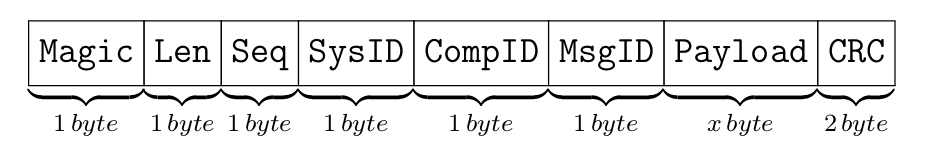
\includegraphics[width=\linewidth]{img/packet.png}
		% Create a subtitle for the figure.
		\caption{Un paquet d'un protocole de communication entre drônes}
		% Define the label of the figure. It's good to use 'fig:title', so you know that the label belongs to a figure.
		\label{fig:packet}
		\end{center}
	\end{figure}
                
        Nous remarquons que plusieurs champs sont ajoutés : 
        \begin{enumerate}
                \item Magic : indique le début de nouveaux messages. 
                \item Length : indique la longueur du champ Payload. Bien que dans notre cas, nous n'en aurions pas besoin car la taille des données échangées est fixe. 
                \item Component ID : représente l'identifiant du composant qui a envoyé ce message. Ce champ pourrait être repris si des couches supplémentaires étaient ajoutées avec des nouvelles 
                fonctionnalités.
                \item Message ID : est l'identifiant du message qui représenterait le type de message transmis : un Heartbeat, une requête de mission, ... Pour notre protocole, nous n'avons pas besoin 
                de ce champ vu qu'un Heartbeat transmet les informations nécessaires et qu'il n'y a donc pas besoin de faire des requêtes.
                \item Payload : réprésente la donnée brute à envoyer
                \item CRC : représente le checksum de la donnée. Il serait intéressant de reprendre ce champs pour ajouter un aspect d'intégrité à notre protocole.
        \end{enumerate}


% Main Part
\section{Résultats}
        Comparons sur différents points notre solution avec un réseau \textit{normal}, c'est à dire un routeur central et 4 noeuds connectés à celui-ci : 

        \textbf{Latence} Celle-ci est relativement faible car nous utilisons UDP et qu'il n'y a pas d'overhead de routage étant donné que nous utilisons
        le Broadcast. Toutefois, cela dépendra de la charge du réseau, du nombre de noeuds "floodant" le réseau et aussi de la constante d'envoi d'Hearbeat. 
        La latence du réseau normal serait légérement plus élevée que celle vue plus haut étant donné que l'information doit parcourir quelques routeurs avant d'arriver à destination. Mais 
        étant donné que les noeuds ne flooderaient pas constamment le réseau, celle-ci pourrait être plus faible. 

        \textbf{Scalabilité} Ce protocole a été imaginé pour des petits réseaux et ne sera pas tenable pour de larges réseaux. 
        Quant au réseau normal, il pourrait acceuillir encore de nombreux appareils (cela dépend évidemment du matériel intégré ainsi que de la bande passante disponible) mais serait 
        limité à un certain nombre à partir duquel la saturation se ferait ressentir.

        \textbf{Robustesse} Ce protocole n'est pas très robuste si on imagine le pire cas, dans lequel par exemple tous les noeuds broadcasteraient en même 
        temps, cela donnerait des mauvaises performances.
        En ce qui concerne le réseau normal, cela dépendrait de plusieurs facteurs comme le protocole de transport utilisé dans les différentes requêtes, il serait plus robuste si TCP est utilisé étant donné les mécanismes mis en place 
        (pas ou peu de surcharge pour le receveur et le réseau). Toutefois, si nous imaginons le pire cas où le routeur central tomberait en panne, c'est tout le réseau qui s'effondrerait.  

        \textbf{Mises à jour périodiques} Un Hearbeat est envoyé toutes les 2 secondes. Quant aux vérifications, elles sont effectuées toutes les 30 secondes. 
        Pour le réseau normal, cela dépend du protocole de routage utilisé, dans notre cas il s'agit d'OSPF, les mises à jour, qui donnent des informations sur les routeurs voisins 
        atteignables, se font toutes les 30 minutes. 

        \textbf{Avantages} Ce protocole est facile à implémenter et convient pour le matériel à notre disposition. Par ailleurs, le système de tracking 
        est assez complet. Enfin, le système est modulaire, ce qui permet de rajouter facilement de nouvelles fonctionnalités à l'aide de nouvelles couches.  

        \textbf{Désavantages} Les inconvénients de ce protocole sont les suivants : premièrement, le réseau est surchargé de messages redondants, ce qui peut 
        causer des collisions et des pertes de paquets (\textit{blind flooding}). Deuxièmement, il n'y a pas de sécurité sur les données, tant au niveau de l'intégrité 
        que de la protection de celles-ci. 

        Nous pouvons le constater, notre protocole est loin d'être parfait même s'il répond au problème initial.

\section{Conclusion}
        Nous avons donc réussi à implémenter un protocole de communication entre les noeuds pouvant s'échanger diverses informations, comme la position ainsi que l'heure liée à cette position. 
        Certes cette version du protocole n'est pas robuste et a ses désavantages mais elle fonctionne sur les petits réseaux et est facile à implémenter. \\

        Pour les futures recherches, il serait intéressant d'améliorer les $2$ fragilités non-négligeables de cette version du protocole sur le long terme, 
        c'est à dire la restructuration du réseau sous forme d'ensembles afin de limiter au maximum le nombre de Broadcasts dans le réseau, mais aussi la sécurité des données. 
        Par ailleurs, il serait intéressant de tester cela avec du matériel plus puissant (avec des antennes dédiées et des drônes à disposition) et de faire un comparatif de performances avec les 
        différents matériels physiques.

\section{Remerciements}
        Je tiens à remercier mon superviseur Nassim Versbraegen pour son aide apportée dans ce rapport et sa présence dans le projet en général.
        Je voudrais également remercier mon collègue Mark Diamantino Caribé pour ses conseils lors de la rédaction de ce rapport. \newpage

\bibliographystyle{unsrt}
\bibliography{bibliography}

\newpage
		
\appendices

% Your document ends here!
\end{document}